\subsection{CURIE (Scientific Long-Context Understanding, Reasoning and Information Extraction)}
{{\footnotesize
\noindent CURIE is a benchmark of 580 problems across six scientific disciplines-materials
science, quantum computing, biology, chemistry, climate science, and astrophysics-
designed to evaluate LLMs on long-context understanding, reasoning, and information 
extraction in realistic scientific workflows.


\begin{description}[labelwidth=4cm, labelsep=1em, leftmargin=4cm, itemsep=0.1em, parsep=0em]
  \item[date:] 2024-04-02
  \item[version:] 1
  \item[last\_updated:] 2024-04-02
  \item[expired:] false
  \item[valid:] yes
  \item[valid\_date:] 2024-04-02
  \item[url:] \href{https://arxiv.org/abs/2503.13517}{https://arxiv.org/abs/2503.13517}
  \item[doi:] 10.48550/arXiv.2503.13517
  \item[domain:] Multidomain Science
  \item[focus:] Long-context scientific reasoning
  \item[keywords:]
    - long-context
    - information extraction
    - multimodal
  \item[licensing:] Apache 2.0 License
  \item[task\_types:]
    - Information extraction
    - Reasoning
    - Concept tracking
    - Aggregation
    - Algebraic manipulation
    - Multimodal comprehension
  \item[ai\_capability\_measured:]
    - Long-context understanding and scientific reasoning
  \item[metrics:]
    - Accuracy
  \item[models:]
    - unkown
  \item[ml\_motif:]
    - Scientific problem solving
  \item[type:] Benchmark
  \item[ml\_task:]
    - Supervised Learning
  \item[solutions:] 0
  \item[notes:] Good
  \item[contact.name:] Subhashini Venugopalan
  \item[contact.email:] vsubhashini@google.com
  \item[datasets.links.name:] unknown
  \item[datasets.links.url:] \href{unknown}{unknown}
  \item[results.links.name:] unknown
  \item[results.links.url:] \href{unknown}{unknown}
  \item[fair.reproducible:] True
  \item[fair.benchmark\_ready:] True
  \item[id:] curie\_scientific\_long-context\_understanding\_reasoning\_and\_information\_extraction
  \item[Citations:] \cite{cui2025curieevaluatingllmsmultitask}
\end{description}

{\bf Ratings:} ~ \\

\begin{tabular}{p{0.15\textwidth} p{0.07\textwidth} p{0.7\textwidth}}
\hline
Rating & Value & Reason \\
\hline
dataset & 4 & Dataset is available via Github, but hard to find
 \\
documentation & 5 & Associated paper explains all criteria
 \\
metrics & 5 & Quantitiative metrics such as ROUGE-L and F1 used. Metrics are tailored to the specific problem.
 \\
reference\_solution & 1 & Exists, but is not open
 \\
software & 4 & Code is available, but not well documented
 \\
specification & 1 & Explains types of problems in detail, but does not state exactly how to administer them.
 \\
\hline
\end{tabular}

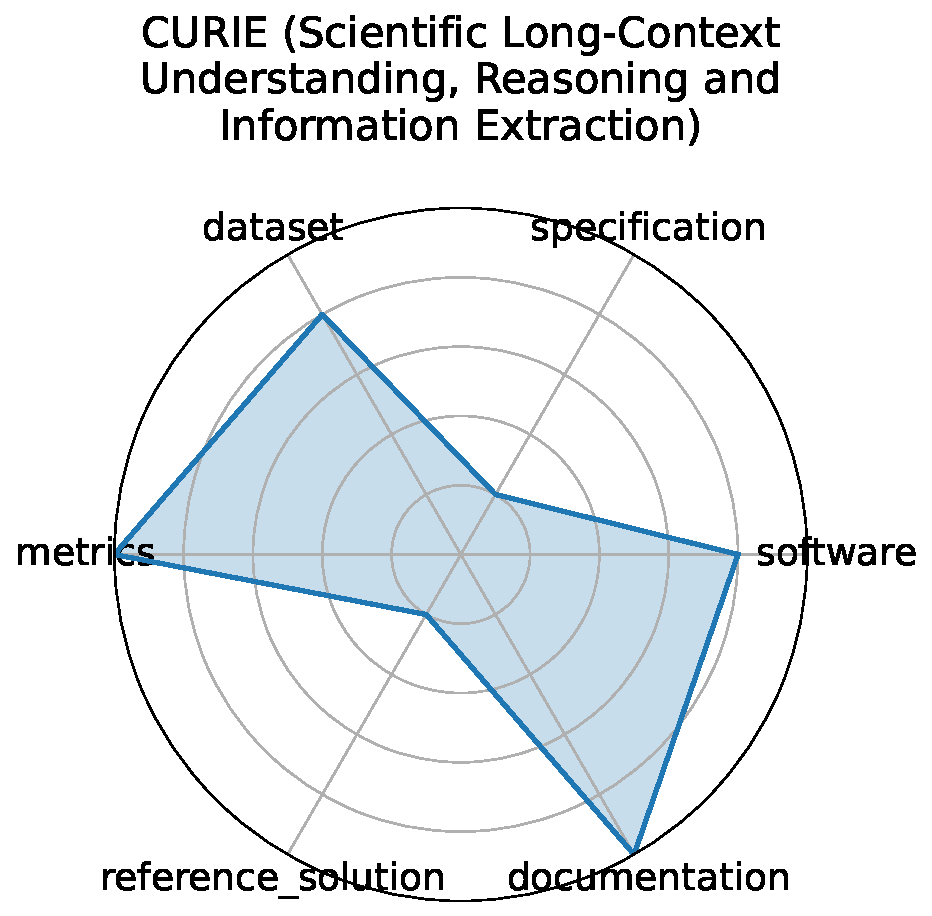
\includegraphics[width=0.2\textwidth]{curie_scientific_long-context_understanding_reasoning_and_information_extraction_radar.pdf}
}}
\clearpage